\documentclass[openany]{book}

\usepackage[margin=1in]{geometry}
\usepackage{amsmath,amsfonts,amsthm, amssymb}
\usepackage{yhmath}
\usepackage{mathrsfs}
\usepackage{mathtools}
\usepackage{xcolor}
\usepackage{graphicx}
\usepackage{comment}
\usepackage{tikz-cd}
\usepackage{quiver}
\usepackage[T1]{fontenc}
\usepackage[utf8]{inputenc}
\usepackage{hyperref}
\renewcommand{\familydefault}{ppl}
\newcommand{\R}{\mathbb{R}}
\newcommand{\C}{\mathbb{C}}
\newcommand{\E}{\mathbb{E}}
\newcommand{\Z}{\mathbb{Z}}
\newcommand{\CC}{\mathcal{C}}
\newcommand{\F}{\mathbb{F}}
\newcommand{\la}{\langle}
\newcommand{\ra}{\rangle}
\newcommand{\colim}{\text{colim}}
\DeclareMathOperator{\im}{im}
\let\oldemptyset\emptyset
\let\emptyset\varnothing
\newcommand{\tor}{\text{Tor}}
\newcommand{\id}{\text{id}}
\newcommand{\ext}{\text{Ext}}
\newcommand{\ptop}{\text{PTop}}
\newcommand{\pt}{\text{pt}}
\newcommand{\ach}{\text{Ach}}


\usepackage{thmtools,thm-restate}

% Fixing mdframed skip below
% See https://tex.stackexchange.com/a/292090/143086
\usepackage[framemethod=TikZ]{mdframed}
\usepackage{xpatch}
\makeatletter
\xpatchcmd{\endmdframed}
	{\aftergroup\endmdf@trivlist\color@endgroup}
	{\endmdf@trivlist\color@endgroup\@doendpe}
	{}{}
\makeatother

\definecolor{huilightpink}{HTML}{fcf2f9}
\definecolor{huidarkpink}{HTML}{ed34b3}
\declaretheoremstyle[
	mdframed={
		backgroundcolor=huilightpink,
		linecolor=huidarkpink,
		rightline=false,
		topline=false,
		bottomline=false,
		linewidth=2pt,
		innertopmargin=5pt,
		innerbottommargin=8pt,
		innerleftmargin=8pt,
		leftmargin=-2pt,
		skipbelow=2pt,
		nobreak
	},
	headfont=\normalfont\bfseries\color{huidarkpink}
]{huipinkbox}
\declaretheorem[style=huipinkbox,name=Theorem,within=chapter]{thm}
\declaretheorem[style=huipinkbox,name=Theorem,sibling=thm]{theorem}





\definecolor{huilightyellow}{HTML}{fff5d6}
\definecolor{huidarkyellow}{HTML}{fcad03}
\declaretheoremstyle[
	mdframed={
		backgroundcolor=huilightyellow,
		linecolor=huidarkyellow,
		rightline=false,
		topline=false,
		bottomline=false,
		linewidth=2pt,
		innertopmargin=5pt,
		innerbottommargin=8pt,
		innerleftmargin=8pt,
		leftmargin=-2pt,
		skipbelow=2pt,
		nobreak
	},
	headfont=\normalfont\bfseries\color{huidarkyellow}
]{huiyellowbox}
\declaretheorem[style=huiyellowbox,name=Proposition,within=chapter]{prop}

\definecolor{huilightpurple}{HTML}{faf2ff}
\definecolor{huidarkpurple}{HTML}{912ed9}
\declaretheoremstyle[
	mdframed={
		backgroundcolor=huilightpurple,
		linecolor=huidarkpurple,
		rightline=false,
		topline=false,
		bottomline=false,
		linewidth=2pt,
		innertopmargin=5pt,
		innerbottommargin=8pt,
		innerleftmargin=8pt,
		leftmargin=-2pt,
		skipbelow=2pt,
		nobreak
	},
	headfont=\normalfont\bfseries\color{huidarkpurple}
]{huipurplebox}
\declaretheorem[style=huipurplebox,name=Lemma,within=chapter]{lem}


\definecolor{huilightpurple}{HTML}{faf2ff}
\definecolor{huidarkpurple}{HTML}{912ed9}
\declaretheoremstyle[
	mdframed={
		backgroundcolor=huilightpurple,
		linecolor=huidarkpurple,
		rightline=false,
		topline=false,
		bottomline=false,
		linewidth=2pt,
		innertopmargin=5pt,
		innerbottommargin=8pt,
		innerleftmargin=8pt,
		leftmargin=-2pt,
		skipbelow=2pt,
		nobreak
	},
	headfont=\normalfont\bfseries\color{huidarkpurple}
]{huipurplebox}
\declaretheorem[style=huipurplebox,name=Definition,within=chapter]{defn}

\definecolor{huilightblue}{HTML}{edf9ff}
\definecolor{huidarkblue}{HTML}{4b79db}
\declaretheoremstyle[
	mdframed={
		backgroundcolor=huilightblue,
		linecolor=huidarkblue,
		rightline=false,
		topline=false,
		bottomline=false,
		linewidth=2pt,
		innertopmargin=5pt,
		innerbottommargin=8pt,
		innerleftmargin=8pt,
		leftmargin=-2pt,
		skipbelow=2pt,
		nobreak
	},
	headfont=\normalfont\bfseries\color{huidarkblue}
]{huiblueblox}
\declaretheorem[style=huiblueblox,name=Example,within=chapter]{example}

\declaretheoremstyle[
	mdframed={
		backgroundcolor=huilightblue,
		linecolor=huidarkblue,
		rightline=false,
		topline=false,
		bottomline=false,
		linewidth=2pt,
		innertopmargin=5pt,
		innerbottommargin=8pt,
		innerleftmargin=8pt,
		leftmargin=-2pt,
		skipbelow=2pt,
		nobreak
	},
	headfont=\normalfont\bfseries\color{huidarkblue}
]{huiblueblox}
\declaretheorem[style=huiblueblox,name=Problem,within=chapter]{prob}

\newcommand{\nirwarnsymbol}{%
	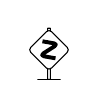
\begin{tikzpicture}[baseline=(x.base)]
		\draw[rounded corners=.01em] (-.05em,-1.07em)rectangle(.05em,.78em);
		\draw[fill=white,rounded corners=1.3] (0,.75em)--(.75em,0)--(0,-.75em)--(-.75em,0)--cycle;
		\draw[line width=0.2mm, line cap=round](-.4em,-1.07em)--(.4em,-1.07em);
		\node(x) at (0,0em) {};
		% Thank you https://tex.stackexchange.com/a/262510
		\draw[
			line cap=but,
			line join=round,
			x=.5em,
			line width=0.5mm,
			y=1*(height("Z")-\pgflinewidth)*(1-sin(10)),
			rotate=-10,
			rounded corners=1.5pt,
		](-0.57, 0.57) -- (0.57, 0.57) -- (-0.57, -0.57) -- (0.57, -0.57);
	\end{tikzpicture}%
}

%%%%%%%%%%%%%%%%%%%%%%%%%%%%%%%%%%%%%%%%%%%% MARGINS
\usepackage{marginnote}
% Thank you https://tex.stackexchange.com/a/472882
% Makes marginnotes always appear on the left, apparently
%
\makeatletter
\long\def\@mn@@@marginnote[#1]#2[#3]{%
	\begingroup
		\ifmmode\mn@strut\let\@tempa\mn@vadjust\else
			\if@inlabel\leavevmode\fi
			\ifhmode\mn@strut\let\@tempa\mn@vadjust\else\let\@tempa\mn@vlap\fi
		\fi
		\@tempa{%
			\vbox to\z@{%
				\vss
				\@mn@margintest
				\if@reversemargin\if@tempswa
						\@tempswafalse
					\else
						\@tempswatrue
				\fi\fi

					\llap{%
						\vbox to\z@{\kern\marginnotevadjust\kern #3
							\vbox to\z@{%
								\hsize\marginparwidth
								\linewidth\hsize
								\kern-\parskip
								%\mn@parboxrestore
								\marginfont\raggedleftmarginnote\strut\hspace{\z@}%
								\ignorespaces#1\endgraf
								\vss
							}%
							\vss
						}%
						\if@mn@verbose
							\PackageInfo{marginnote}{xpos seems to be \@mn@currxpos}%
						\fi
						\begingroup
							\ifx\@mn@currxpos\relax\else\ifx\@mn@currpos\@empty\else
									\kern\@mn@currxpos
							\fi\fi
							\ifx\@mn@currpage\relax
								\let\@mn@currpage\@ne
							\fi
							\if@twoside\ifodd\@mn@currpage\relax
									\kern-\oddsidemargin
								\else
									\kern-\evensidemargin
								\fi
							\else
								\kern-\oddsidemargin
							\fi
							\kern-1in
						\endgroup
						\kern\marginparsep
					}%
			}%
		}%
	\endgroup
}
\makeatother
%
% Mostly for todonotes
\renewcommand{\marginpar}{\marginnote}
%%%%%%%%%%%%%%%%%%%%%%%%%%%%%%%%%%%%%%%%%%%% /MARGINS

\definecolor{nirlightred}{RGB}{250, 220, 220}
\definecolor{nirdarkred}{HTML}{f40000}
\declaretheoremstyle[
	mdframed={
		backgroundcolor=nirlightred,
		linecolor=nirdarkred,
		rightline=false,
		topline=false,
		bottomline=false,
		linewidth=2pt,
		innertopmargin=5pt,
		innerbottommargin=8pt,
		innerleftmargin=8pt,
		leftmargin=-2pt,
		skipbelow=2pt,
		nobreak
	},
	headfont=\normalfont\bfseries\color{nirdarkred}
]{nirredbox}

% \makeatletter
% \declaretheorem[
% 	style=nirredbox,
% 	name=Warning,
% 	sibling=thm,
% 	% without \leavevmode, the first item in a list gets misformatted
% 	postheadhook={\leavevmode\marginnote{\nirwarnsymbol}[-3pt]%
% 	\ifthmt@thisistheone% restatable makes alignment weird
% 		\hspace{-2.2pt}%
% 	\fi}
% ]{warn}
% \makeatother

\newcommand{\nirideasymbol}{%
	
\begin{tikzpicture}[baseline=(x.base)]
		\draw[rounded corners=.01em] (-.05em,-1.07em)rectangle(.05em,.78em);
		\draw[fill=white,rounded corners=1.3] (0,.75em)--(.75em,0)--(0,-.75em)--(-.75em,0)--cycle;
		\draw[line width=0.2mm, line cap=round](-.4em,-1.07em)--(.4em,-1.07em);
		\node(x) at (0,0em) {};
		\node at (0,0em) {{\textbf{!}}};
	\end{tikzpicture}%
}
\renewcommand{\nirwarnsymbol}{%
	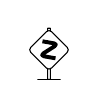
\begin{tikzpicture}[baseline=(x.base)]
		\draw[rounded corners=.01em] (-.05em,-1.07em)rectangle(.05em,.78em);
		\draw[fill=white,rounded corners=1.3] (0,.75em)--(.75em,0)--(0,-.75em)--(-.75em,0)--cycle;
		\draw[line width=0.2mm, line cap=round](-.4em,-1.07em)--(.4em,-1.07em);
		\node(x) at (0,0em) {};
		% Thank you https://tex.stackexchange.com/a/262510
		\draw[
			line cap=but,
			line join=round,
			x=.5em,
			line width=0.5mm,
			y=1*(height("Z")-\pgflinewidth)*(1-sin(10)),
			rotate=-10,
			rounded corners=1.5pt,
		](-0.57, 0.57) -- (0.57, 0.57) -- (-0.57, -0.57) -- (0.57, -0.57);
	\end{tikzpicture}%
}
\makeatletter
\declaretheorem[
	style=nirredbox,
	name=Idea,
	sibling=thm,
	% without \leavevmode, the first item in a list gets misformatted
	postheadhook={\leavevmode\marginnote{\nirideasymbol}[-3pt]%
	\ifthmt@thisistheone% restatable makes alignment weird
		\hspace{-2.2pt}%
	\fi}
]{idea}

\declaretheorem[
	style=nirredbox,
	name=Warning,
	sibling=thm,
	% without \leavevmode, the first item in a list gets misformatted
	postheadhook={\leavevmode\marginnote{\nirwarnsymbol}[-3pt]%
	\ifthmt@thisistheone% restatable makes alignment weird
		\hspace{-2.2pt}%
	\fi}
]{warn}
\makeatother

\title{$L^2$ Estimate of the Schrodinger Maximal Function}

\date{\today}
\author{Xiumin Du, Ruixiang Zhang}

\begin{document}

\maketitle

\tableofcontents



\newpage

This is based on the paper \textcolor{red}{insert paper} and Xiumin Du's ICM 2022 talk.

\chapter{Background}
We first recall Carleson's pointwise convergence problem for the Schrodinger equation. In this portion, we will discuss
\begin{enumerate}
    \item Schrodinger maximal estimates
    \item Comparison with Fourier restriction conjecture.
\end{enumerate}
In the second part, we will discuss a generalization of the Schrodinger estimates, which are called weighted Fourier extension estimates. These weighted restriction estimates have several applications:
\begin{enumerate}
    \item Divergence set of Schrodinger solutions
    \item Spherical average Fourier decay rates of fractal measures
    \item Falconer's distance set problem
\end{enumerate}

\section{Introduction to Carleson's pointwise convergence problem}
\begin{defn}[Fourier transform, Fourier inversion]
Let $g:\R^n\to\C$, the Fourier transform of $g$ is defined as 
\begin{equation*}
    \hat{g}(\xi)=\int_{\R^n}g(x)e^{-ix\cdot\xi}dx
\end{equation*}
Fourier inversion formula states that $g$ can be recovered via the inverse transform:
\begin{equation*}
    g(x)=(2\pi)^{-n}\int_{\R^n}\hat{g}(\xi)e^{ix\cdot\xi}d\xi
\end{equation*}
\end{defn}
We recall the free Schrodinger equation:
\begin{equation*}
    \begin{cases}
        iu_t+\Delta u=0, (x,t)\in\R^n\times\R\\
        u(x,0)=f(x), x\in\R^n
    \end{cases}
\end{equation*}
applying Fourier transform with respect to $x$ to both sides, we get the following ODE in $t$:
\begin{equation*}
    i\frac{\partial}{\partial t}\hat{u}(\xi, t)-|\xi|^2(\xi,t)=0
\end{equation*}
solving this ODE and plugging in initial data, and applying the Fourier inversion formula we have 
\begin{equation*}
    u(x,t)=(2\pi)^{-n}\int_{\R^n}e^{i(x\cdot\xi+t|\xi|^2)}\hat{f}(\xi)d\xi:=e^{it\Delta}f(x)
\end{equation*}
We recall some basic facts about these solutions.
\begin{prop}(Properties of $e^{it\Delta}f(x)$)
    Let $e^{it\Delta}f(x)$ be defined as above, i.e., the solutions to the free Schrodinger problem with initial data $f(x)$, the following are true:
    \begin{enumerate}
        \item (Conservation of energy) $\|e^{it\Delta}f(x)\|_{L^2(\R^n)}=\|f\|_{L^2(\R^2)}$ for any $t$.
        \item (Convergence in $L^2$) $\lim_{t\to 0}\|e^{it\Delta}f(x)-f(x)\|_{L^2(\R^n)}=0$ for all $f\in L^2$.
        \item $\lim_{t\to 0}e^{it\Delta}f(x)=f(x)$ a.e. fails for some $f\in L^2$. 
    \end{enumerate}
\end{prop}
The last question is central to this talk: what regularity of $f$ is required to ensure pointwise convergence?
\begin{equation*}
    \lim_{t\to 0}e^{it\Delta}f(x)=f(x)
\end{equation*}
we will zoom this ``regularity'' in Sobolev spaces. 
\begin{defn}[Sobolev space, norm]
    For integer $k$, 
    \begin{equation*}
        H^k(\R^n)=\{f\in L^2(\R^n):D^{\alpha}f\in L^2 \text{ for each multi-index} \alpha \text{ with }|\alpha|\leq k\}
    \end{equation*}
    One can see that $f\in H^k(\R^n)$ if and only if
    \begin{equation*}
        \|f\|_{H^k}:=\left(\int_{\R^n}(1+|\xi|^2)^k|\hat{f}(\xi)|^2d\xi\right)^2<\infty
    \end{equation*}
    Thus we generalize to arbitrary $s\in\R$: define the Sobolev space $H^s$ as 
    \begin{equation*}
        H^s(\R^n)=\left\{f\in L^2(\R^n): \|f\|_{H^s}<\infty\right\}
    \end{equation*}
    where 
    \begin{equation*}
        \|f\|_{H^s}:=\left(\int_{\R^n}(1+|\xi|^2)^s|\hat{f}(\xi)|^2d\xi\right)^2
    \end{equation*}
    where $s$ is called the order of regularity.
\end{defn}
\section{History of Carleson's pointwise convergence problem}
Carleson (1979) proposed the following pointwise convergence problem:
\begin{prob}[Carleson, 1979]
    Determine the minimal $s$ such that if $f\in H^s(\R^n)$, then 
    \begin{equation}\label{PC}
        \lim_{t\to 0}e^{it\Delta}f(x)=f(x) \tag{PC}
    \end{equation}
\end{prob}
The known results are as follows: when $n=1$
\begin{enumerate}
    \item Carleson 1979: (PC) holds for $s\geq\frac{1}{4}$, in $n=1$.
    \item Dahlber-Kenig 1981: (PC) fails if $s<\frac{1}{4}$, for all $n$. In other words, Carleson's result is sharp in $n=1$.
\end{enumerate}
In higher dimensions,
\begin{enumerate}
    \item Sjolin, Vega 1987: (PC) holds for $s>\frac{1}{2}$, for all $n\geq 2$. This is later improved by Bourgain, Moya-Vargas-Vega, Tao-Vargas, \dots
    \item S. Lee 2006: (PC) holds for $s>\frac{3}{8}$ when $n=2$.
    \item Bourgain 2012: (PC) holds for $s>\frac{1}{2}-\frac{1}{4n}$ for all $n\geq 2$.
    \item Bourgain 2012: (PC) fails if $s<\frac{1}{2}-\frac{1}{n}$ for all $n>4$. 
    \item Bourgain 2016: (PC) fails if $s<\textcolor{red}{\frac{n}{2(n+1)}}=\frac{1}{2}-\frac{1}{2(n+1)}$, for all $n\geq 2$. 
    \item Du-Guth-Li 2017: (PC) holds for $s>\textcolor{red}{1/3}$ when $n=2$. This is sharp up to the endpoint.
    \item Du-Zhang 2019: (PC) holds for $s>\textcolor{red}{\frac{n}{2(n+1)}}$ for all $n\geq 3$. This is sharp up to the endpoint.
\end{enumerate}
The resolution of (PC) uses deep results from Fourier restriction in harmonic analysis. Before we discuss these techniques, we discuss its connection to the Fourier restriction conjecture.

\begin{prob}[Stein's Fourier restriction problem,  1978]
    For $h\in L^p$, can one meaningfully restrict $\hat{h}$ to the truncated parabloid $S=\{(\xi,|\xi|^2:\xi\in B^n(0,1))\}$? More explicity, for which $p,q$ does the following hold:
    \begin{equation*}
        \left(\int_S|\hat{h}(\xi)|^qd\sigma(\xi)\right)^\frac{1}{q}\leq C\|f\|_{L^p}
    \end{equation*}
    where $d\sigma(\xi, |\xi|^2)=d\xi$ is the surface measure. By duality, this question can be formulated as asking for $p,q$ such that 
    \begin{equation*}
        \|\mathcal{E}g\|_{L^p}\leq C\|g\|_{L^q}
    \end{equation*}
    where $\mathcal{E}$ is the extension 
    operator for the paraboloid
    \begin{equation*}
        \mathcal{E}(g)(x)=\frac{1}{(2\pi)^n}\int_{B^{n-1}}e^{i(x'\cdot\omega+x_n|\omega|^2)}f(\omega)d\omega
    \end{equation*}
    where $x=(x',x_n)\in\R^n$.
\end{prob}
The motivation is as follows: if $h\in L^1(\R^n)$, then $\hat{h}$ is continuous and bounded, therefore can be restricted to any subset.  If $h\in L^2$, then $\hat{h}\in L^2$, therefore cannot be meaningfully restricted to Lebesgue measure zero subsets (hypersurfaces). Stein asked for $h\in L^p$ where $1<p<2$, can we meaningfully restrict $\hat{f}$ to a hypersurface $S$ (e.g. the sphere $\mathbb{S}^{n-1})$ such that $\hat{f}\vert_S$ in some $L^q$ space?


One can express the solution to the Schrodinger solution in terms of the Fourier extension operator:
\begin{align*}
    u^{it\Delta}f(x)&=(2\pi)^{-n}\int_{\R^n}e^{i(x\cdot\xi+t|\xi|^2)}\hat{f}(\xi)d\xi\\
    &=\mathcal{E}(\hat{f})(x,t)
\end{align*}
We now list some landmark results that influence the progress of the (PC):
\begin{enumerate}
    \item{} [Wolff, 1996], [Tao, 2003]: Bilinear restriction estimates, established (PC) for $s>\frac{3}{8}$ when $n=2$.
    \item{} [Bennett-Carbery-Tao, 2006]:  Multilinear restriction estimates 
    \item{} [Bourgain-Guth, 2011]: From multilinear restriction estimates to a linear one, using induction on dimensions and different scales, established (PC) for $s>\frac{1}{2}-\frac{1}{4n}$ for all $n$. 
    \item{} [Bourgain-Demeter, 2015]: $l^2$ decoupling theorem.
    \item{} [Guth, 2016]: A restriction estimates using polynomial partitioning, which is essential for the final resolution for (PC).
\end{enumerate}
Recall that 
\begin{equation*}
    \lim_{t\to 0}e^{it\Delta}f(x)=f(x) \text{ for all  }f\in H^s(\R^n)
\end{equation*}
is a consequence of the following estimate of the Schrodinger maximal function: for $f\in H^s$, 
\begin{equation*}
    \left\|\sup_{0<t\leq 1}|e^{it\Delta}f|\right\|_{L^2(B^n(0,1))}\leq C_s\|f\|_{H^s(\R^n)}
\end{equation*}
We can further reduce this via Littlewood-Paley decomposition, parabolic rescaling and localizaion using wave packets, it suffices to show 
\begin{equation*}
    \left\|\sup_{0<t\leq 1}|e^{it\Delta}f|\right\|_{L^2(B^n(0,R))}\lessapprox R^\frac{n}{2(n+1)}\|f\|_{L^2}\tag{SME}
\end{equation*}
where $A\lessapprox B$ iff $A\leq C_\varepsilon R^\varepsilon B$ for any $\varepsilon>0$ and $R\geq 1$. (SME stands for Schrodinger maximal estimates).

\begin{thm}(Du, et.al, )
    \begin{equation*}
        \left\|\sup_{0<t<\leq R}|e^{it\Delta}f(x)||\right\|_{L^3(B_R^2)}\lessapprox \|f\|_2
    \end{equation*}
    for all $f$ with $\text{supp}\hat{f}\subset B_1^2$. 
\end{thm}

\begin{thm}[Du-Zhang, 2019] 
    (SME) holds in dimension $n+1$.
\end{thm}
Next, we will compare the Schrodinger maximal estimates and the Fourier restriction conjecture. We will use the locally constant property. 
\begin{prop}[Locally constant property]
    Suppose $f$ is such that $\text{supp}\hat{f}\subset B^n(0,1)$, let $B$ be any unit tube in $\R^{n+1}$. (White lie: $|e^{it\Delta}f(x)|$ is essentially constant on $B$). Rigorously, 
    \begin{equation*}
        \|e^{it\Delta}f(x)\|_{L^1(B)}\lesssim\|e^{it\Delta}f(x)\|_{L^\infty(B)}\lesssim\|e^{it\Delta}f(x)\|_{L^1(\omega(B))}
    \end{equation*}
    where $\omega\sim 1$ on $B$ and rapidly decaying off $B$.
\end{prop}
We recall the Fourier restriction conjecture:
\begin{equation*}
    \|e^{it\Delta}f(x)\|_{L^3(B_R^3, dxdt)}\lessapprox \|\hat{f}\|_\infty
\end{equation*}
for all $f: \text{supp}\hat{f}\subset B_1^2$. 
\begin{enumerate}
    \item By locally constant property, $\|e^{it\Delta}f(x)\|_{L_x^3L_t^\infty}\lesssim \|e^{it\Delta}f(x)\|_{L_x^3L_t^3}$
    \item By Plancherel, $\|f\|_2\lesssim\|\hat{f}\|_\infty$, since $\hat{f}$ has compact support.
\end{enumerate}
Thus the both sides of SME are less than those of the restriction conjecture. While SME is settled, the restriction conjecture still remains (wildly) open. 

Now we write down the weighted $L^2$ estimate proven by Du-Zhang. We say $Y$ is an $\alpha$-dimensional set in $B_R^{n+1}$, provided that $Y$ is a union of lattice unit cubes in $B_R^{n+1}$ s.t. 
\begin{equation*}
    |Y\cap B^{n+1}(c,r)|\lesssim r^\alpha
\end{equation*}
for all $c$ and $r\geq 1$. We say $H$ is an $\alpha$-dimensional weight in $\R^{n+1}$ if it is a non-negative measurable function on $\R^{n+1}$ that satisfies 
\begin{equation*}
    \int_{B^{n+1}(c,r)}H(y)dy\lesssim r^\alpha, \forall c, \forall r\geq 1
\end{equation*}


















\end{document}